\documentclass[Bachelorarbeit.tex]{subfiles}
\begin{document}

\graphicspath{{./figures/newMarket/}}	%specifying the folder for the figures

\chapter{A new Market}
\label{ch:newMarket}
As already introduced in section \ref{ch:interpretation_reenablingTrading} a new market is necessary to repair the miss-allocation of collateralized assets in the range of the pessimist agents by enabling the agents to trade collateralized assets against cash.

\medskip

The initial idea for this market was by the supervisor of this thesis Mr. Hans-Joachim Vollbrecht.

\section{Definition}
\subsection{Products}
Collateralized assets are traded against cash. The buyer gets a specific amount of collateralized assets for a given amount of cash where the seller gives away the specific amount of collateralized assets and gets the given amount of cash.

\subsection{Price-Range}
As with all other three markets the price-ranges of the offers must be defined. Note that all prices must be obviously in the unit of cash according to the previously defined products.

\paragraph{minimum}
When calculating the minimum price of a collateralized asset - that is how much is the collateralized asset minimally worth - it is important to include the collateral-aspect of the asset. Thus one starts with the minimum asset-price in cash which is the down-price \textit{pD} and subtracts the minimum amount of cash which is bound through a bond as collateral which is \textit{pD}. This value is a constant for all agents.

\begin{equation}
min_{collateral} = \textit{pD} - \textit{pD} = 0
\end{equation}
 
\paragraph{maximum}
To calculate the maximum price of a collateralized asset - that is how much is the collateralized asset maximally worth - one needs to include the collateral-aspect of the asset too. Equal to calculating the minimum one starts now with the maximum asset-price in cash which is the up-price \textit{pU} and subtracts the maximum possible amount of cash which is bound through a bond as collateral which is the face-value \textit{V}. This value is a constant for all agents.

\begin{equation}
max_{collateral} = \textit{pU} - \textit{V}
\end{equation}

\paragraph{limit}
Applying the same rules as in minimum and maximum to the limit price calculation one needs to subract the limit-price of bonds from the limit-price of asset to receive the limit-price of a collateralized asset. This value is individual for each agent as the limit-prices differ across the agents both for assets and bonds.

\begin{equation}
limit_{collateral} = limit_{asset} - limit_{loan}
\end{equation}

\subsection{Bid-Offering}
The way bid-offers are generated is very similar to the Bond/Cash market. Bid offers are generated only when the agent has any cash holdings. The price is drawn randomly between the minimum price and the limit-price because when buying one wants to buy below the expected value to make a profit. As amount one TRADING-UNIT of an asset is selected - in the thesis-implementation 0.1 - but if there is not enough cash left to buy one TRADING-UNIT of assets then the amount of assets is selected which can be bought with the remaining cash holdings.

\begin{table}[H]
	\centering
	\caption{Bid-Offering parameters}
	\begin{tabular} { l c r }
		\hline
		Pre-Condition & $\textit{cash holdings} > 0$  \\
		Asset-Price & $\mathrm{random}(min_{collateral}, limit_{collateral})$ \\
		Asset-Amount & $\min ( \frac{ \textit{cash holdings} }{ \textit{asset-price} }, \textit{TRADING-UNIT} )$ \\
		\hline
	\end{tabular}
\end{table}


\subsection{Ask-Offering}
The way ask-offers are generated is very similar to the Bond/Cash market. Ask offers are generated only when the agent has any collateralized assets. The price is drawn randomly between the limit-price and maximum price because when selling one wants to sell above the expected value to make a profit. As amount one TRADING-UNIT of an asset is selected - in the thesis-implementation 0.1 - but if there are fewer collateralized assets left then the remaining amount of collateral is selected.
See chapter \ref{ch:implementation} for the equation of the amount of collateralized assets.

\begin{table}[H]
	\centering
	\caption{Ask-Offering parameters}
	\begin{tabular} { l c r }
		\hline
		Pre-Condition & $\textit{collateral} > 0$  \\
		Asset-Price & $\mathrm{random}(\textit{limit-price of coll. asset}, \textit{max coll. asset-price})$ \\
		Asset-Amount & $\min ( { \textit{collateralized assets} }, \textit{TRADING-UNIT} )$ \\
		\hline
	\end{tabular}
\end{table}

\subsection{Match}
Below the wealth-exchange table is given in case of a match between two agents on the new market. Note that the wealth is increased/decreased as given by the +/- signs.

\begin{table}[H]
	\centering
	\caption{Wealth-Exchange on match}
	\begin{tabular} { l c c }
		& Seller & Buyer \\
		\hline
		Loans Given & + matching-amount & N/A \\
		Loans Taken & N/A & - matching-amount \\
		Assets holdings & - matching-amount & + matching-amount \\
		Cash holdings  & + matching-price & - matching-price \\
		\hline
	\end{tabular}
\end{table}

Note that regarding these formulas it is clear that the Collateral/Cash market can't work without the BP-mechanism because only with it is it allowed to increment the net-loans variable \textit{loan} by incrementing \textit{loans given}. Without the BP-mechanism incrementing \textit{loans given} would simply be forbidden thus making this market unable to work. Because of this the thesis has the BP-mechanism hard-wired into the implementation and does not provide the user with an option to run the simulation without it.

\section{Results}
The plain results of the simulation with using the new market are given in this section where the interpretation of the results are given in the following one.

\medskip

As experiment-configuration the same is used as given in chapter \ref{ch:results} except that the new market is now activated too.

\begin{table}[H]
	\centering
	\caption{Configuration for all experiments}
	\begin{tabular} { l c r }
		\hline
		Agent-Count & 100 \\
		Bond-Type & 0.5 \\
		Replication-Count & 50 \\
		Matching-Round & max. 500 offering-rounds \\
		Terminate after & 1000 failed successive matching-rounds \\
		\hline
	\end{tabular}
\end{table}

\subsection{Fully-Connected topology}

\begin{figure}[H]
	\centering
  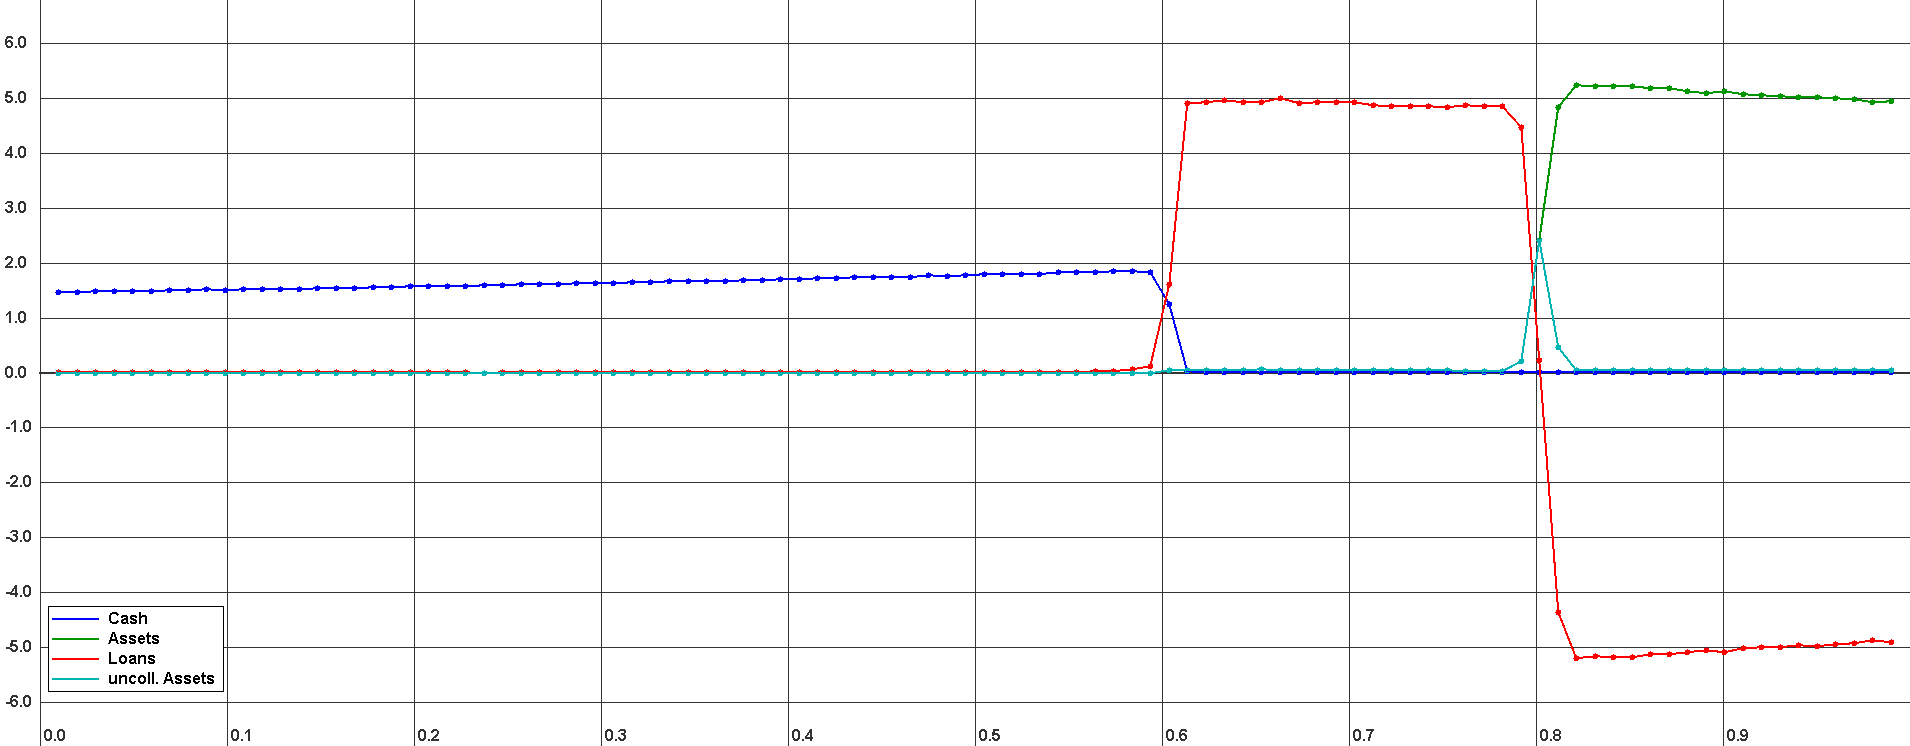
\includegraphics[width=1.0\textwidth, angle=0]{FULLYCONNECTED_100_WITHCOLLATERALMARKET_REPL.png}
	\caption{Wealth-Distribution of Fully-Connected topology with Collateral/Cash market enabled.}
	\label{fig:wealth_FULLYCONNECTED_100_WITHCOLLATERALMARKET_REPL}
\end{figure}

\begin{table}[H]
	\caption{Equilibrium of Fully-Connected topology with Collateral/Cash market enabled}
	\label{tab:equilibrium_FULLY_CONNECTED_WITH_COLLATERALCASH}
	\centering
	\begin{tabular} { l c r }
		\hline
		Asset-price p & 0.718 (0.016) \\
		Bond-price q & 0.383 (0.000) \\
		Marginal agent i1 & 0.603 (0.003) \\
		Marginal agent i2 & 0.812 (0.000) \\
		\hline
		Pessimist wealth & 1.640 (0.002) \\
		Medianist wealth & 4.808 (0.074) \\
		Optimist wealth & 5.171 (0.023) \\
		\hline
	\end{tabular}
\end{table} 

\begin{table}[H]
	\caption{Performance of Fully-Connected topology with Collateral/Cash market enabled}
	\centering
	\begin{tabular} { l c r }
		\hline
		Successful matching-rounds & 1,803.86 (20.24) \\
		Failed matching-rounds & 1,365.88 (134.63) \\
		Total matching-rounds & 3,169.74 (137.60) \\
		\hline
		Ratio successful/total & 0.57 \\
		Ratio failed/total & 0.43 \\
		\hline
	\end{tabular}
\end{table}

\begin{table}[H]
	\caption{Difference of Fully-Connected topology to theoretical equilibrium as given in Table \ref{tab:theoretical_equilibrium_100Agents_05Bond}}
	\centering
	\begin{tabular} { l c c c r }
		& Result & Reference & difference to Reference \\
		\hline
		Asset-Price p & 0.718 & 0.717 & +0.1\% \\
		Bond-Price q & 0.383 & 0.375 & +2.1\% \\
		Marginal Agent i1 & 0.603 & 0.584 & +3.2\% \\
		Marginal Agent i2 & 0.812 & 0.803 & +1.1\% \\
		\hline
	\end{tabular}
\end{table} 

\begin{table}[H]
	\caption{Difference of Fully-Connected topology to equilibrium without Collateral/Cash market as given in Table \ref{tab:fullyconnected_equilibrium_100Agents_05Bond}}
	\centering
	\begin{tabular} { l c c c r }
		& Result & Reference & difference to Reference \\
		\hline
		Asset-Price p & 0.718 (0.016) & 0.717 (0.015) & +0.1\% (+6.6\%) \\
		Bond-Price q & 0.383 (0.000) & 0.382 (0.001) & +0.2\%  \\
		Marginal Agent i1 & 0.603 (0.003) & 0.596 (0.004) & +1.2\% (-25\%) \\
		Marginal Agent i2 & 0.812 (0.000) & 0.810 (0.004) & +0.24\% \\
		\hline
		Pessimist Wealth & 1.640 (0.002) & 1.646 (0.004) & -0.3\% (-50\%) \\
		Medianist Wealth & 4.808 (0.074) & 4.736 (0.089) & +1.5\% (-16\%) \\
		Optimist Wealth & 5.171 (0.023) & 5.179 (0.082) & -0.1\% (-71\%) \\
		\hline
	\end{tabular}
\end{table} 

\subsection{Ascending-Connected topology}
\begin{figure}[H]
	\centering
  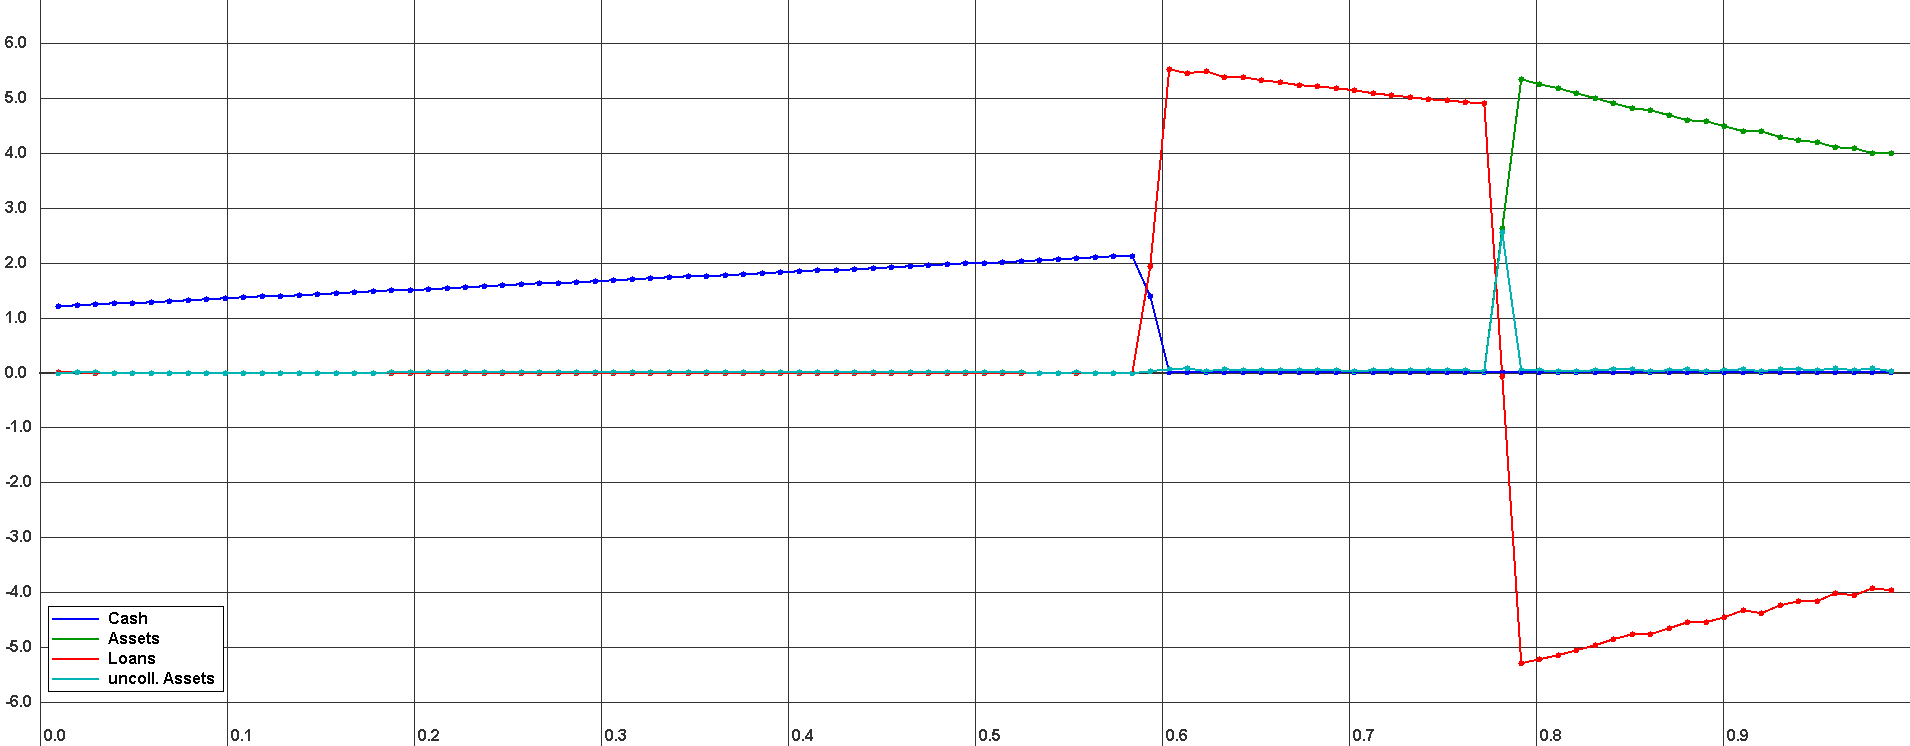
\includegraphics[width=1.0\textwidth, angle=0]{ASCENDINGCONNECTED_100_WITHCOLLATERALMARKET_REPL.png}
	\caption{Wealth-Distribution of Ascending-Connected topology with Collateral/Cash market enabled.}
	\label{fig:wealth_ASCENDINGCONNECTED_100_WITHCOLLATERALMARKET_REPL}
\end{figure}

\begin{table}[H]
	\caption{Equilibrium of Ascending-Connected topology}
	\centering
	\begin{tabular} { l c r }
		\hline
		Asset-price p & 0.729 (0.004) \\
		Bond-price q & 0.380 (0.001) \\
		Marginal agent i1 & 0.594 (0.001) \\
		Marginal agent i2 & 0.792 (0.000) \\
		\hline
		Pessimist wealth & 1.647 (0.003) \\
		Medianist wealth & 4.999 (0.032) \\
		Optimist wealth & 4.581 (0.013) \\
		\hline
	\end{tabular}
\end{table} 

\begin{table}[H]
	\caption{Performance of Ascending-Connected topology}
	\centering
	\begin{tabular} { l c r }
		\hline
		Successful matching-rounds & 48,629.32 (197.20) \\
		Failed matching-rounds & 1,001.30 (1.31) \\
		Total matching-rounds & 49,630.62 (197.30) \\
		\hline
		Ratio successful/total & 0.98 \\
		Ratio failed/total & 0.02 \\
		\hline
	\end{tabular}
\end{table}

\begin{table}[H]
	\caption{Difference of Ascending-Connected topology to theoretical equilibrium as given in Table \ref{tab:theoretical_equilibrium_100Agents_05Bond}}
	\centering
	\begin{tabular} { l c c c r }
		& Result & Reference & difference to Reference \\
		\hline
		Asset-Price p & 0.729 & 0.717 & +1.6\% \\
		Bond-Price q & 0.380 & 0.375 & +1.3\% \\
		Marginal Agent i1 & 0.594 & 0.584 & +1.7\% \\
		Marginal Agent i2 & 0.792 & 0.802 & -1.2\% \\
		\hline
	\end{tabular}
\end{table} 

\begin{table}[H]
	\caption{Difference of Ascending-Connected topology to equilibrium of Fully-Connected topology with Collateral/Cash as given in table \ref{tab:equilibrium_FULLY_CONNECTED_WITH_COLLATERALCASH}}
	\centering
	\begin{tabular} { l c c c r }
		& Result & Reference & difference to Reference \\
		\hline
		Asset-Price p & 0.729 (0.004) & 0.718 (0.016) & +1.5\% (-80\%) \\
		Bond-Price q & 0.380 (0.001) & 0.383 (0.000) & -0.8\% \\
		Marginal Agent i1 & 0.594 (0.001) & 0.603 (0.003) & -1.4\% (-60\%) \\
		Marginal Agent i2 & 0.792 (0.000) & 0.812 (0.000) & -2.4\% \\
		\hline
		Pessimist Wealth & 1.647 (0.003) & 1.640 (0.002) & +0.4\% (+50\%) \\
		Medianist Wealth & 4.999 (0.032) & 4.808 (0.074) & +3.9\% (-56\%) \\
		Optimist Wealth & 4.581 (0.013) & 5.171 (0.023) & -11.4\% (-43\%) \\
		\hline
	\end{tabular}
\end{table}

\section{Interpretation of results}
When interpreting the results the following questions must be answered:

\begin{itemize}
\item Does the Fully-Connected topology reach the theoretical equilibrium as well with Collateral/Cash market enabled?
\item Does the new market repair the miss-allocation of wealth in the pessimists-range of the Ascending-Connected topology?
\item If not why? If yes, does the Ascending-Connected topology approach theoretical equilibrium now?
\end{itemize}

\paragraph{Does the Fully-Connected topology reach the theoretical equilibrium as well with Collateral/Cash market enabled?}
Yes it does. Both visual and statistical results show that it reaches the theoretical equilibrium. The medianist wealth is slightly higher with the new market but that difference, as well as the variations in the other variables are not statistically significant.

\paragraph{Does the new market repair the miss-allocation of wealth in the pessimists-range of the Ascending-Connected topology?}
Yes it does. The visual results are clear with no miss-allocations showing up within 50 replications. If there would have been miss-allocations within any replication they would have shown up in the final result.

\paragraph{If yes, does the Ascending-Connected topology approach theoretical equilibrium now?}
The miss-allocations are repaired but it does does not approach theoretical equilibrium. Both visual and statistical results show that it misses to reach the theoretical and Fully-Connected topology. Although p,q,i1 and i2 do not differ significant the wealth of the optimists and medianists are substantially different and show a different shape than in the Fully-Connected case and thus the theoretical equilibrium is not reached.

\section{Simulation and Market dynamics}
When implementing a new market the market-dynamics are of very importance and thus the following questions must be answered.

\begin{itemize}
\item Can the trading stages 1-4 be identified too as given in \cite{Breuer2015}?
\item How does trading progresses with this new market? Is it the same as without the new market?
\item How does the new market resolve the miss-allocation (with and without deferred activation)?
\item When and how much is each market active? 
\item How do the market-activities change when a new market is introduced?
\end{itemize}

To answer these questions one must look closely at the market-dynamics. There are trading stages to be identified but due to the new market and the different topology they are expected to be quite different from the ones found in \cite{Breuer2015}. The method used to find these stages is through observation of a single run and refining and validating the derived facts over many additional runs. Note that replications provide no real value here as one needs to look very carefully into the dynamics of single runs instead of the mean of multiple runs.

\subsection{Fully-Connected with new Market}

\begin{figure}[H]
	\centering
  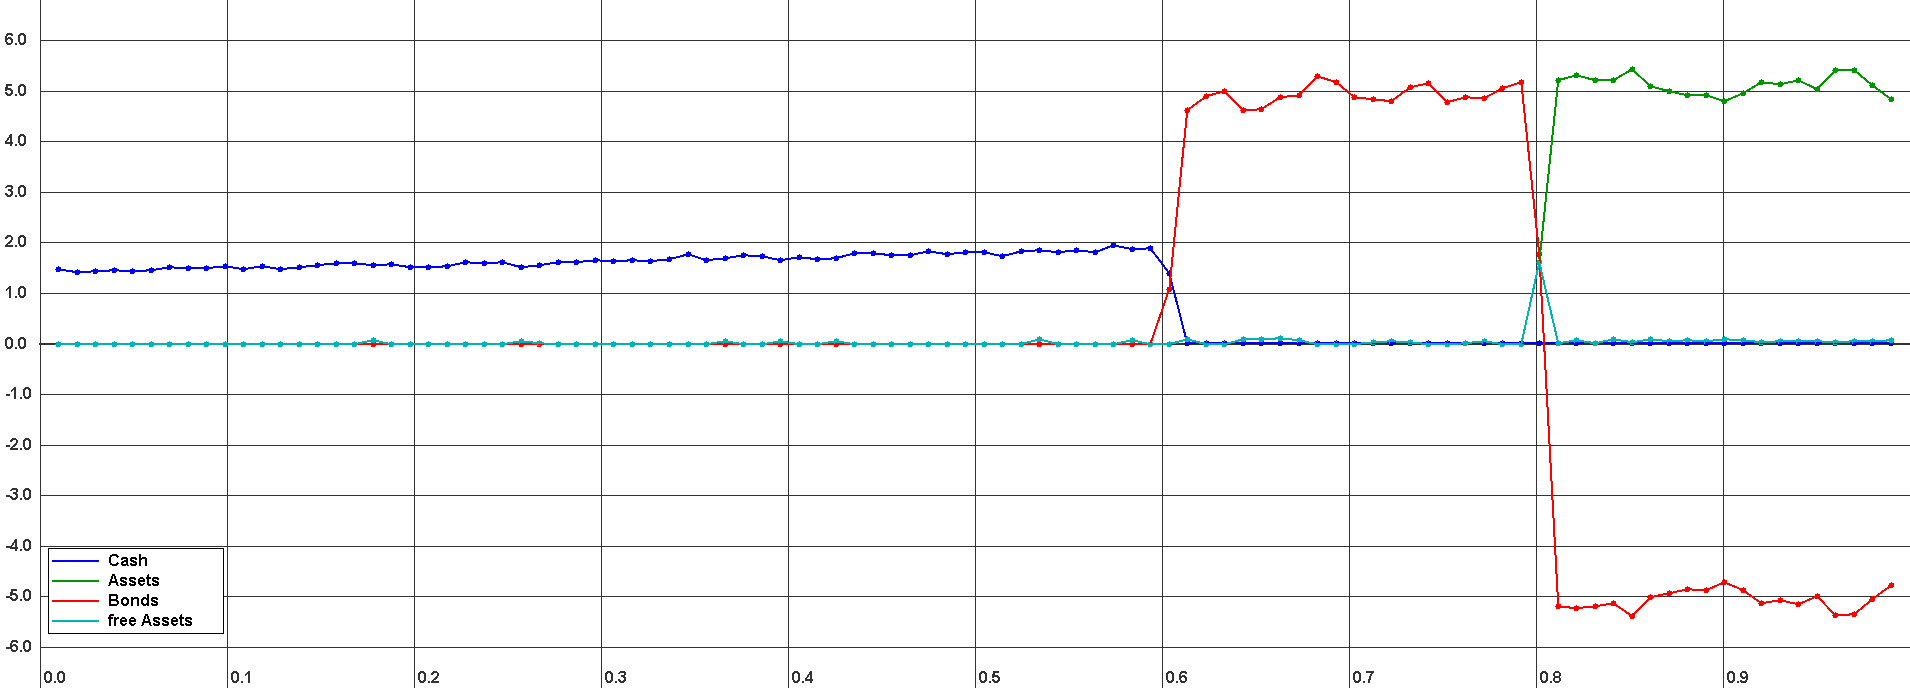
\includegraphics[width=1.0\textwidth, angle=0]{fc/FULLYCONNECTED_100_WITHCOLLATERALMARKET_WEALTH_SINGLE.png}
  	\caption{Final wealth-distribution of a single run of the Fully-Connected topology with Collateral/Cash market.}
	\label{fig:wealth_FULLYCONNECTED_100_WITHCOLLATERALMARKET_WEALTH_SINGLE}
\end{figure}

\begin{figure}[H]
	\centering
  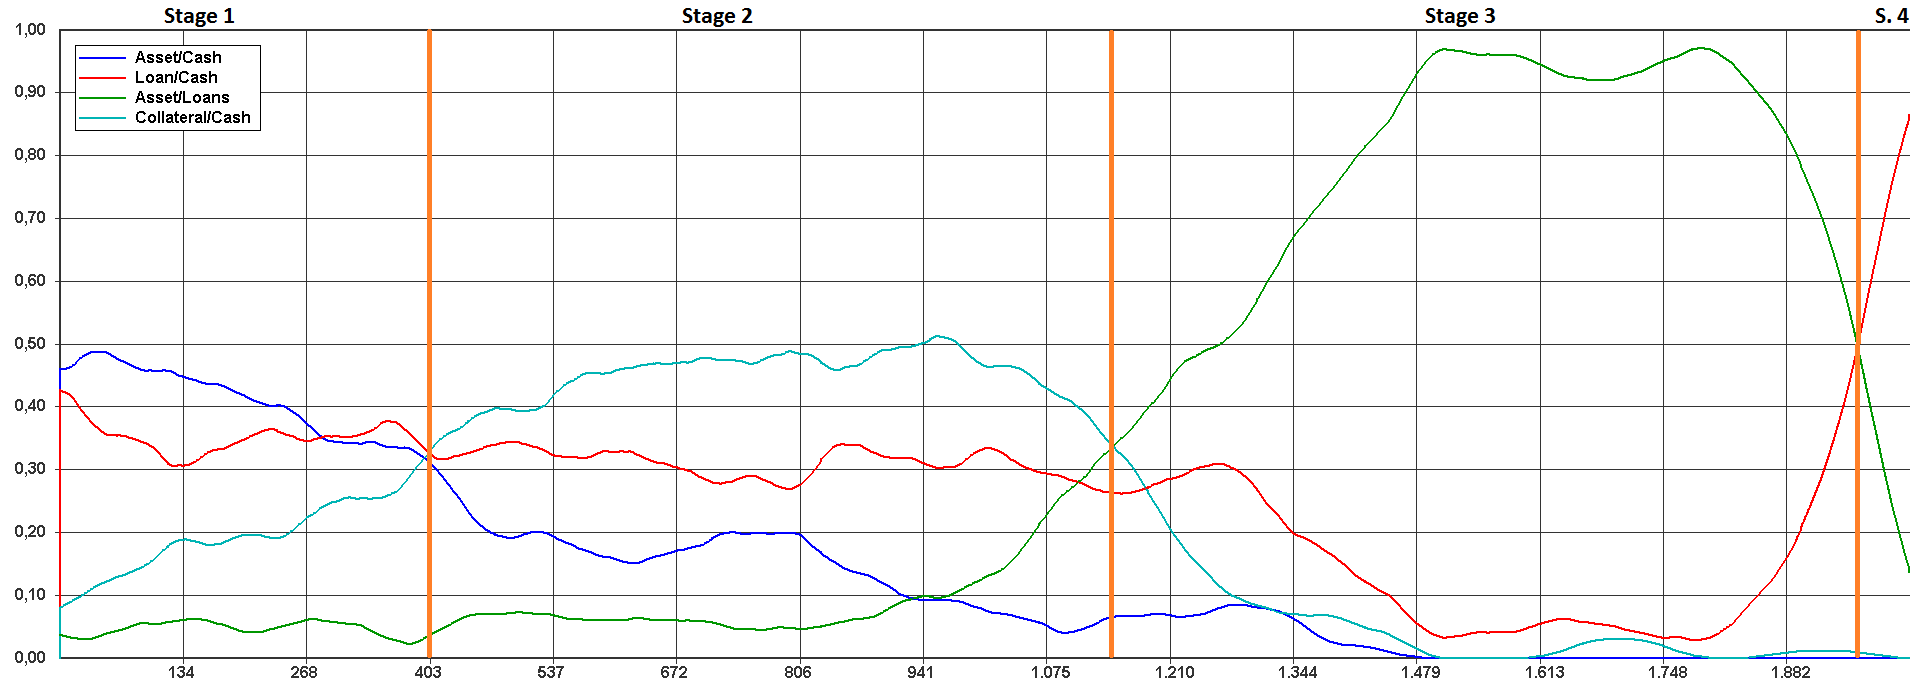
\includegraphics[width=1.0\textwidth, angle=0]{fc/FULLYCONNECTED_100_WITHCOLLATERALMARKET_MARKET_STAGES.png}
  	\caption{Market-activity stages of the single run of figure \ref{fig:wealth_FULLYCONNECTED_100_WITHCOLLATERALMARKET_WEALTH_SINGLE}.}
	\label{fig:markets_FULLYCONNECTED_100_WITHCOLLATERALMARKET_MARKET_STAGES}
\end{figure}

4 Stages were identified which resemble roughly the ones given in \cite{Breuer2015} as the new market doesn't make a big impact due to the fully-connectedness.


\paragraph{Stage 1}
In this stage the pessimists become visible rapidly as they sell their assets and increase their cash wealth. One can get also a sense of the more optimistic range of agents as they gather assets both free and collateralized. The medianists are not visible yet. This picture is in stark contrast to the one given in Ascending-Connected topology where the wealth stabilizes from both the left and right ends towards the marginal agent i2. This is obviously due to the different topology as in the fully-connected one all agents can trade with each other thus the wealth-distribution approaches the theoretical equilibrium over all agents and not only on two frontiers from left and right.

\medskip

The Asset/Cash market dominates but goes down slowly as fewer and fewer pessimists trade assets against cash compared to the very beginning. The Bond/Cash market is slightly increasing as more and more bonds are traded because they remain the alternative method of payment for assets and because the pessimists trade them up towards the optimists using the BP-mechanism. The Collateral/Cash market begins quite low and stays in the range of a 10\% share as it is not heavily required for the pessimists due to the fully-connectedness. The Asset/Bond market starts quite strong and stays at this level as pessimists trade assets with optimists against bonds.

\begin{figure}[H]
	\centering
  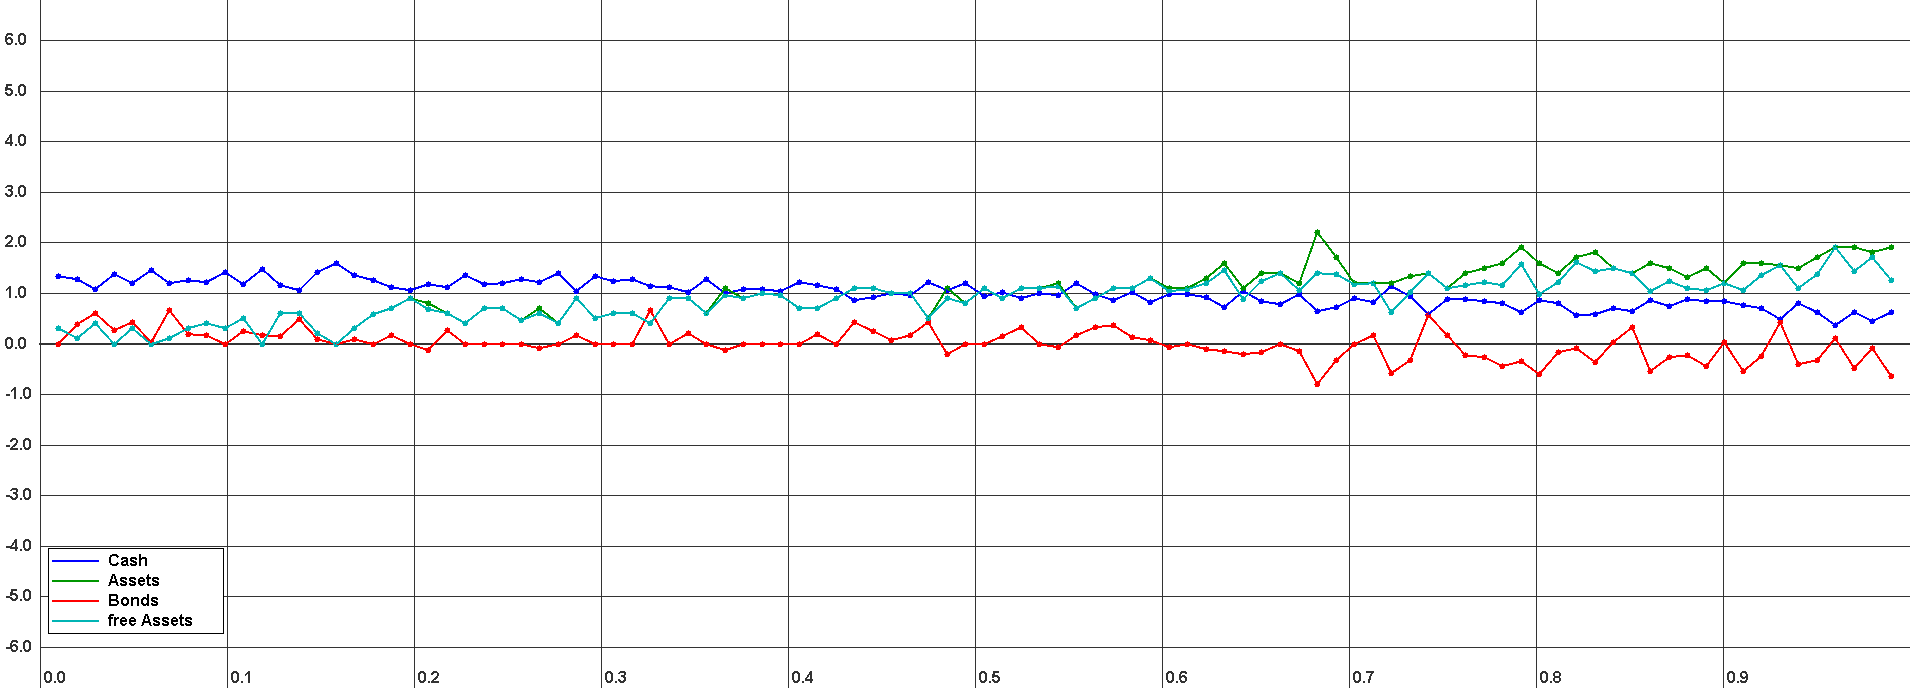
\includegraphics[width=1.0\textwidth, angle=0]{fc/FULLYCONNECTED_100_WITHCOLLATERALMARKET_WEALTH_STAGE_1.png}
  	\caption{Wealth-Distribution during Stage 1 of the single run of figure \ref{fig:wealth_FULLYCONNECTED_100_WITHCOLLATERALMARKET_WEALTH_SINGLE}.}
	\label{fig:markets_FULLYCONNECTED_100_WITHCOLLATERALMARKET_WEALTH_STAGE_1}
\end{figure}

\paragraph{Stage 2}
The bonds, free- and collateralized assets are all traded from the pessimists towards the optimists and the optimists crystallize themselves even more but no medianists are visible yet.

\medskip

The Asset/Cash market continues to go down as the cash holdings of the pessimists begin to decline. The Bond/Cash market raises even further as agents switch to this market because the pessimists have ran out of cash. The Collateral/Cash market is still in the range of the 10\% share because its not really needed in the Fully-Connected topology. The Asset/Bond market raises fast towards the end of the stage as the optimists are then out of cash and need to distribute the collateralized assets between each other and the yet to come medianists.

\begin{figure}[H]
	\centering
  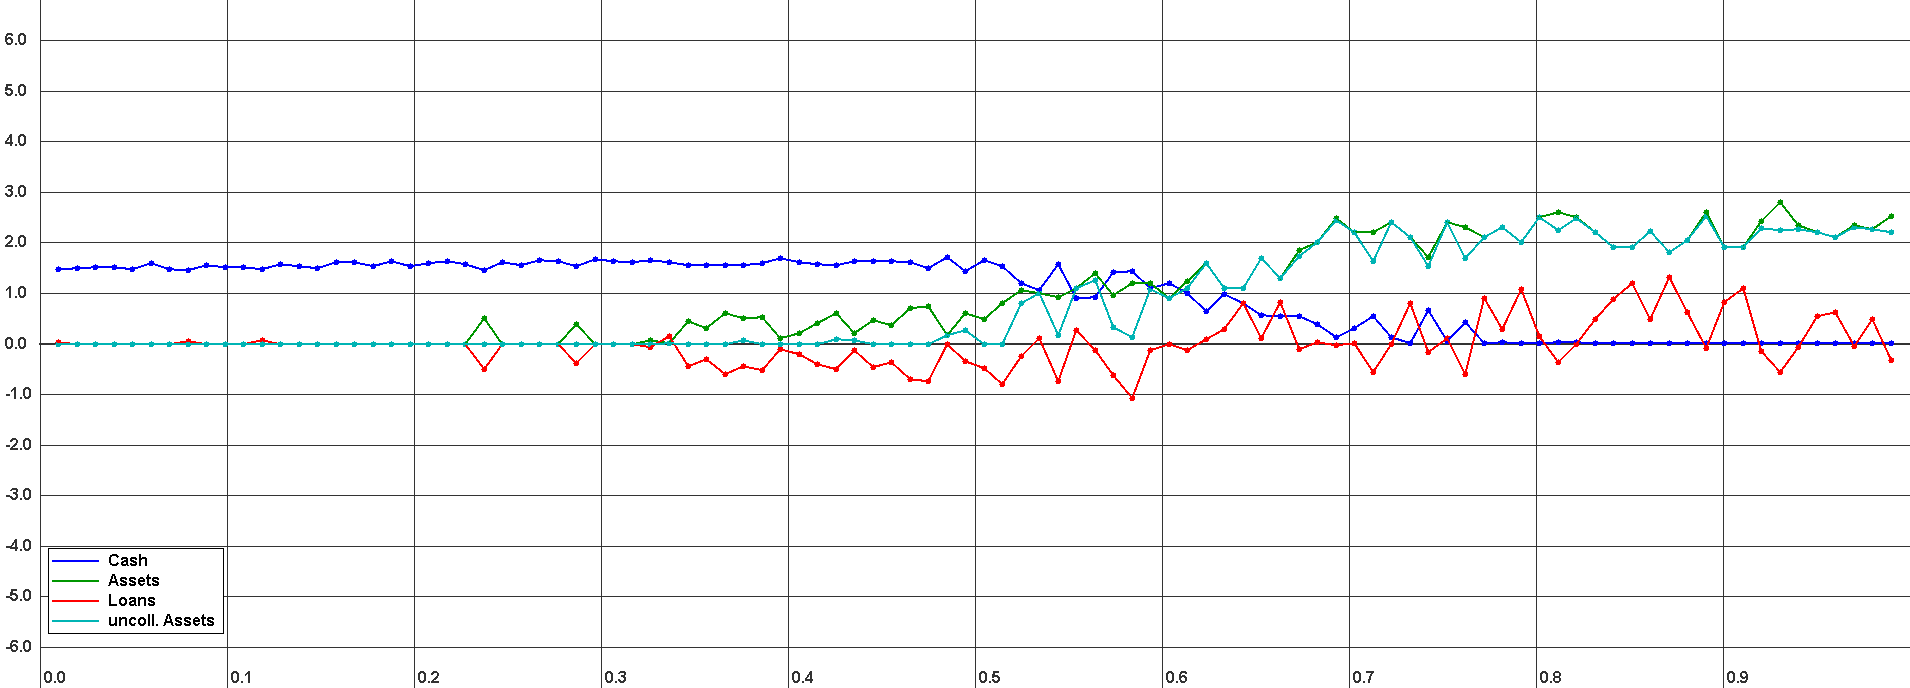
\includegraphics[width=1.0\textwidth, angle=0]{fc/FULLYCONNECTED_100_WITHCOLLATERALMARKET_WEALTH_STAGE_2.png}
  	\caption{Wealth-Distribution during Stage 2 of the single run of figure \ref{fig:wealth_FULLYCONNECTED_100_WITHCOLLATERALMARKET_WEALTH_SINGLE}.}
	\label{fig:markets_FULLYCONNECTED_100_WITHCOLLATERALMARKET_WEALTH_STAGE_2}
\end{figure}

\paragraph{Stage 3}
The pessimists are now nearly inactive as only the more optimistic pessimists hold a few bonds which they trade towards the now emerging medianists. The i1-point is beginning to show up but is not yet refined. 

\medskip

Because the pessimists are nearly inactive now and hold no more assets and cash the Asset/Cash and Collateral/Cash markets go down and decline completely. The Bond/Cash market goes down but does not decline as bonds are still traded because of the emerging of medianists. The medianists and pure optimists which are emerging have no other possibility than to trade on the Asset/Bond market to further distribute their collateralized assets among each other which is the reason for the rise of the Asset/Bond market above all others and its heavy domination. Despite the heavy domination of the Asset/Bond market still a few bonds are traded against cash between the most optimistic pessimists and the medianist to refine the i1 point.

\begin{figure}[H]
	\centering
  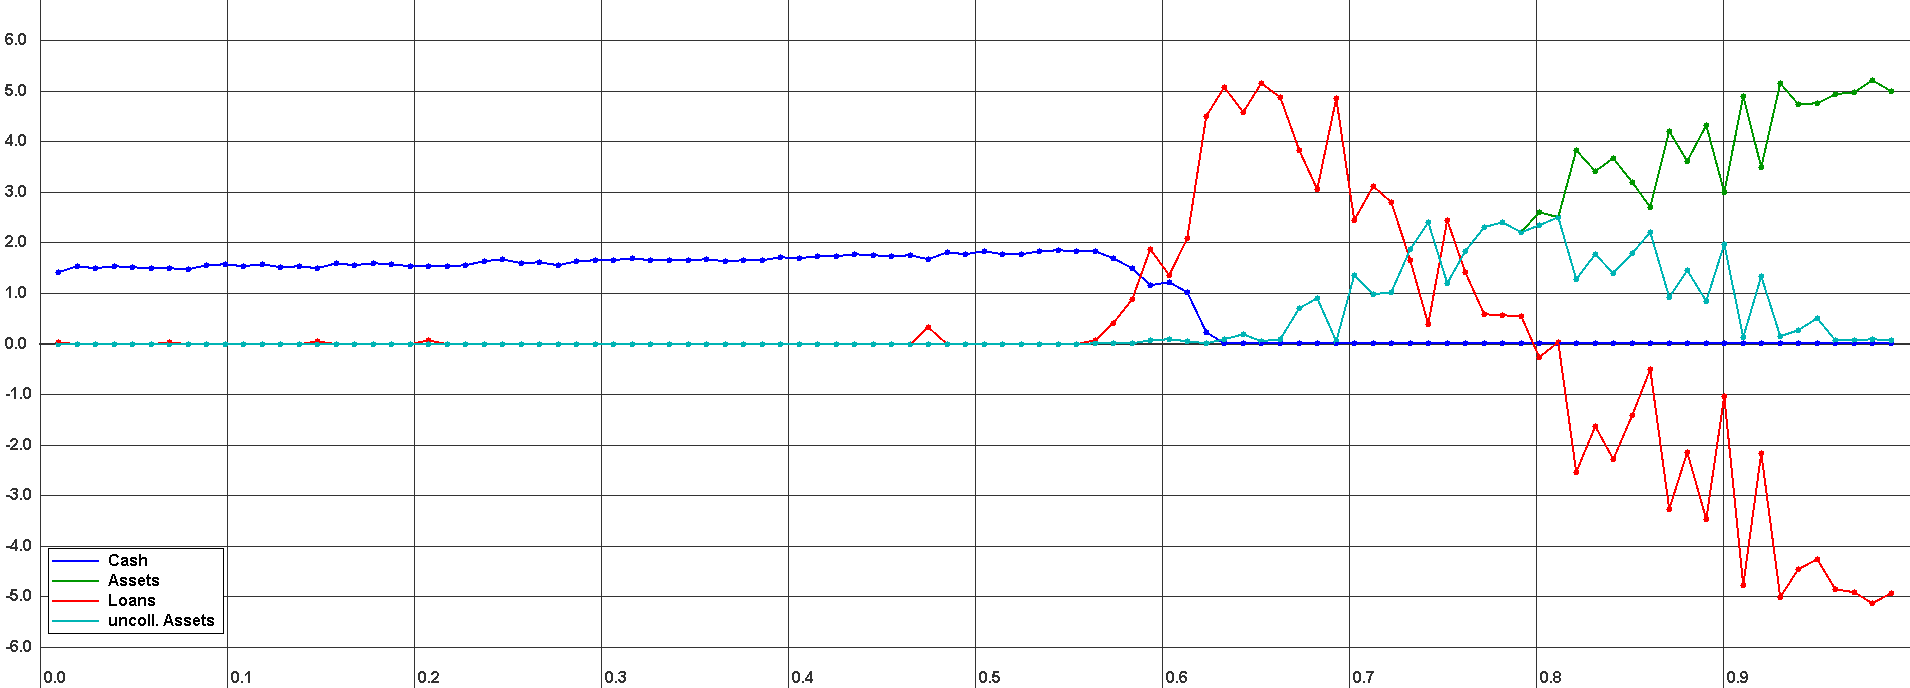
\includegraphics[width=1.0\textwidth, angle=0]{fc/FULLYCONNECTED_100_WITHCOLLATERALMARKET_WEALTH_STAGE_3.png}
  	\caption{Wealth-Distribution during Stage 3 of the single run of figure \ref{fig:wealth_FULLYCONNECTED_100_WITHCOLLATERALMARKET_WEALTH_SINGLE}.}
	\label{fig:markets_FULLYCONNECTED_100_WITHCOLLATERALMARKET_WEALTH_STAGE_3}
\end{figure}

\paragraph{Stage 4}
The pessimists are finally inactive except a couple of most optimistic pessimists around the i1 point which still trade with the medianists on the Bond/Cash market to refine the i1 point to the final allocation as can be seen in figure \ref{fig:wealth_FULLYCONNECTED_100_WITHCOLLATERALMARKET_WEALTH_SINGLE}. Also the i2 is now emerging and a couple of medianists and optimists are trading around it on the Asset/Bond market to achieve the final allocation.

\medskip

Only the Bond/Cash and Asset/Bond markets are active any more. The Bond/Cash market is active due to the final transactions between the most optimistic pessimists which want to sell their final bonds to the medianists which is only possible through cash which the most pessimistic medianists still own. The Asset/Bond market is active due to the final transactions between the most optimistic medianists which want to sell their free assets to the optimists which is only possible through bonds because the most pessimistic optimists have no more cash left thus they have to trade assets against bonds.

\begin{figure}[H]
	\centering
  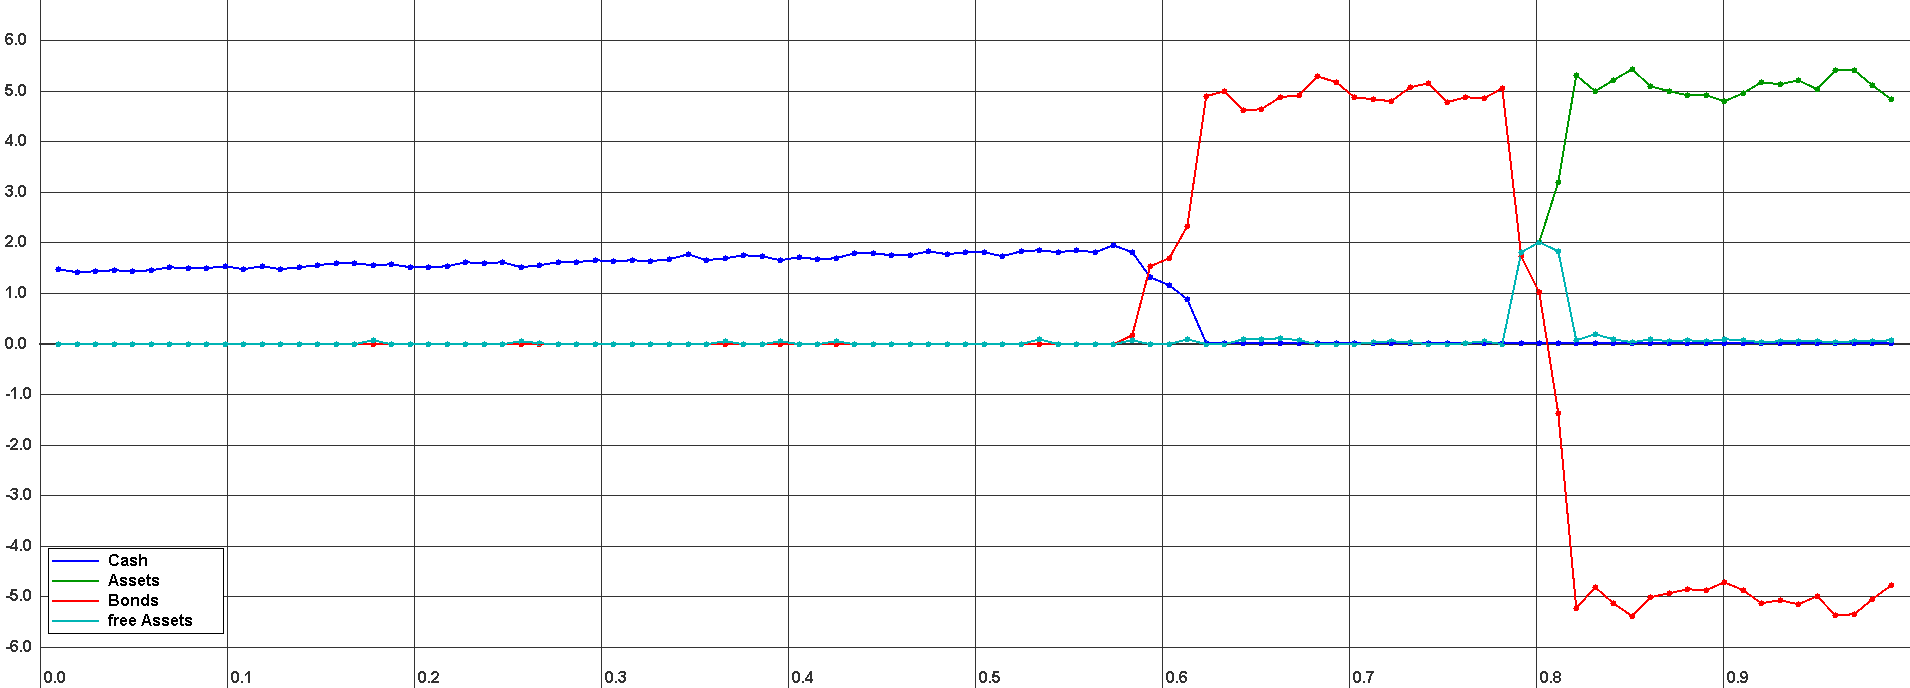
\includegraphics[width=1.0\textwidth, angle=0]{fc/FULLYCONNECTED_100_WITHCOLLATERALMARKET_WEALTH_STAGE_4.png}
  	\caption{Wealth-Distribution during Stage 4 of the single run of figure \ref{fig:wealth_FULLYCONNECTED_100_WITHCOLLATERALMARKET_WEALTH_SINGLE}.}
	\label{fig:markets_FULLYCONNECTED_100_WITHCOLLATERALMARKET_WEALTH_STAGE_4}
\end{figure}

\subsection{Deferred new market enabling}
Using the thesis-software it is possible to start a simulation-run with Ascending-Connected topology without the Collateral/Cash market and enabling it after 1,000 successive failed matching-rounds which gives interesting hints about how the spikes of collateralized assets in the pessimists-range are resolved and distributed over the already existing pure optimists.

\medskip

\begin{figure}[H]
	\centering
  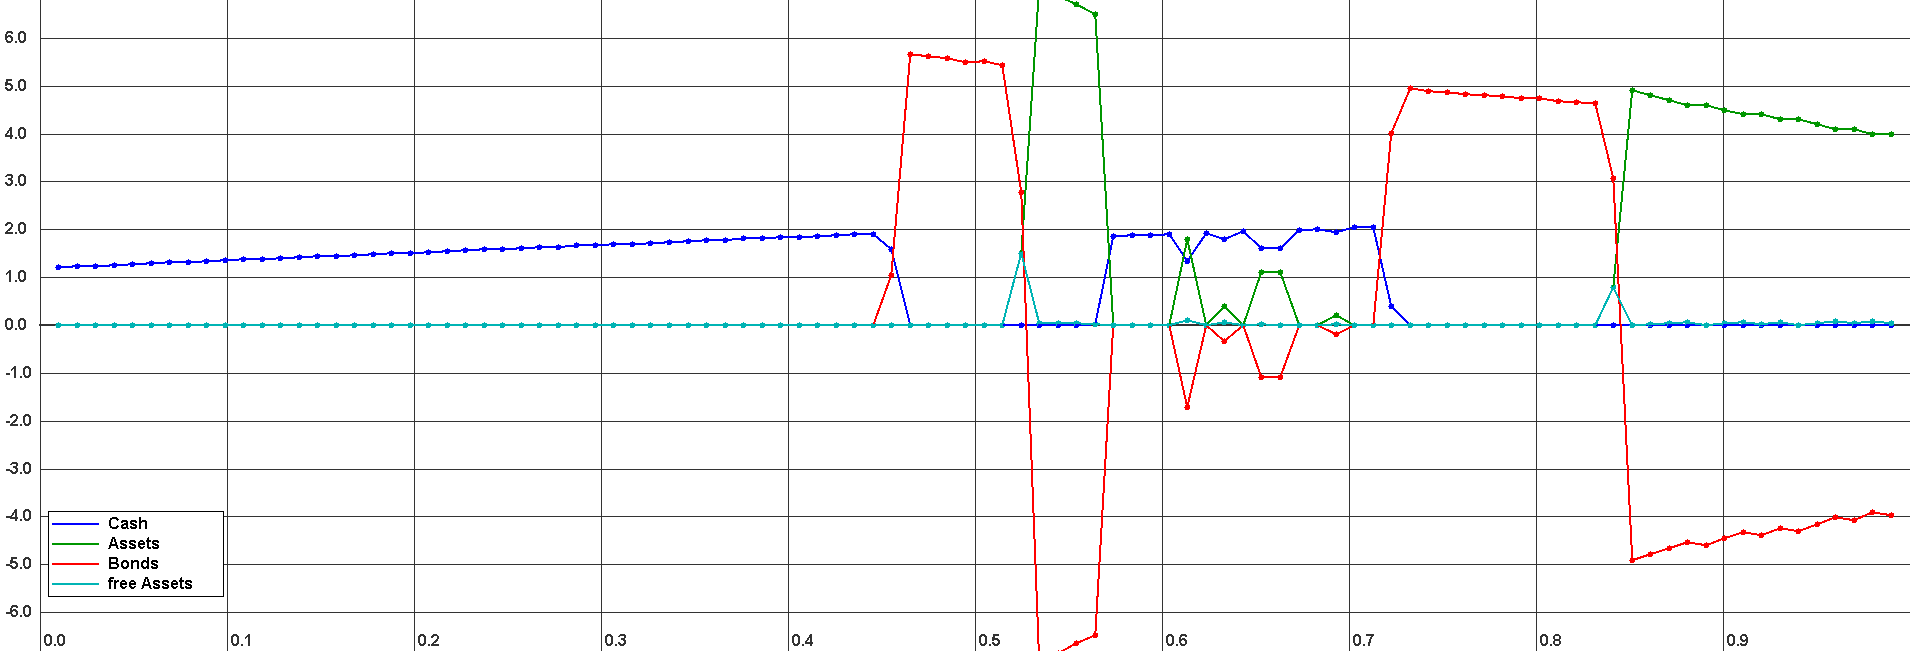
\includegraphics[width=1.0\textwidth, angle=0]{ac/ASCENDINGCONNECTED_100_DEFERREDCOLLATERALMARKET_SINGLE_MISSALLOCATED.png}
  	\caption{Wealth-distribution of a single run of Ascending-Connected topology before enabling the Collateral/Cash market.}
	\label{fig:wealth_ASCENDINGCONNECTED_100_DEFERREDCOLLATERALMARKET_SINGLE_MISSALLOCATED}
\end{figure}

\begin{figure}[H]
	\centering
  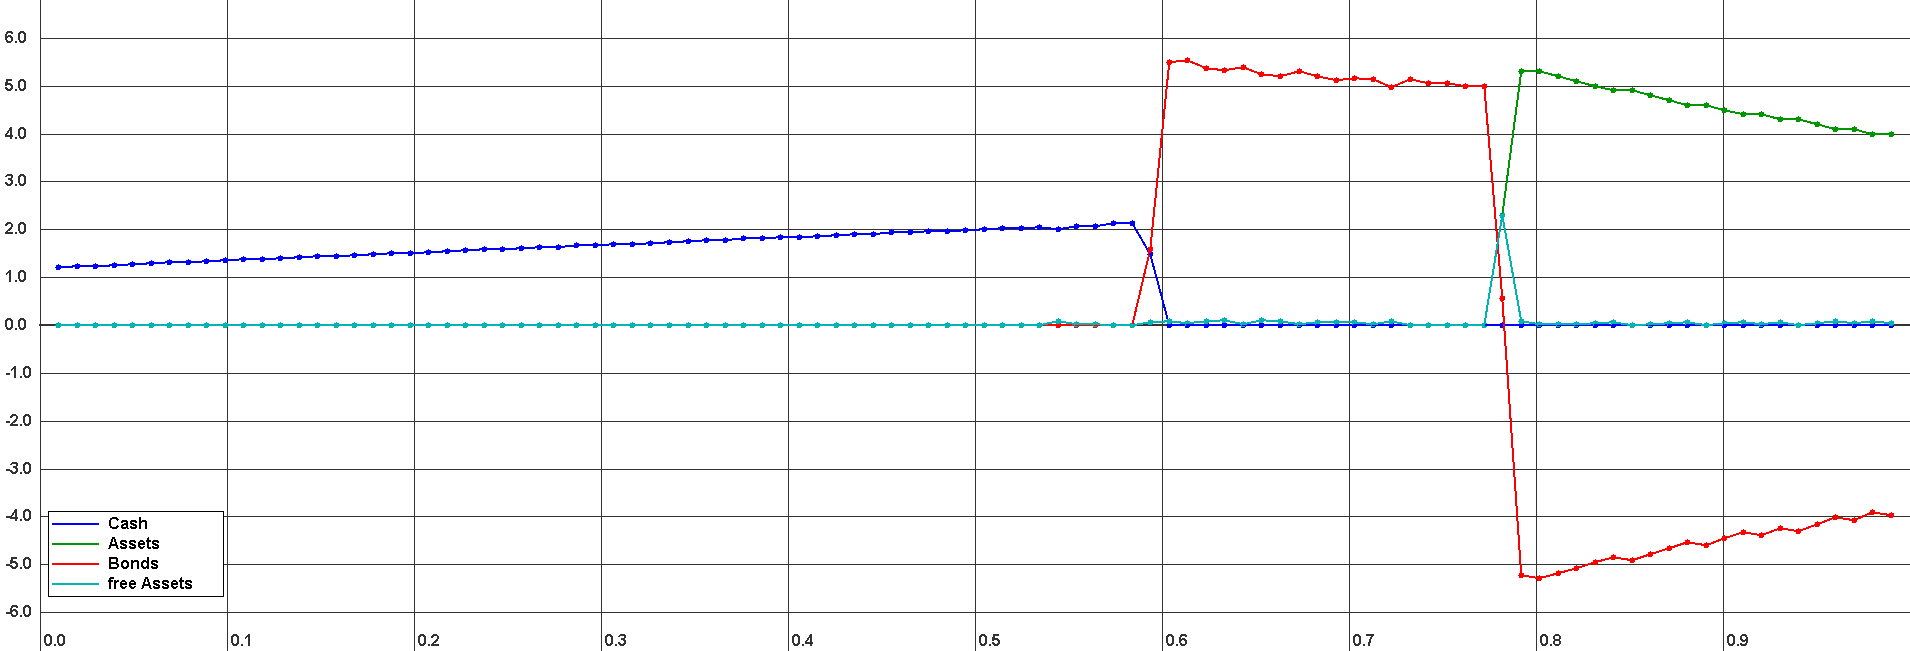
\includegraphics[width=1.0\textwidth, angle=0]{ac/ASCENDINGCONNECTED_100_DEFERREDCOLLATERALMARKET_SINGLE_FINAL.png}
  	\caption{Final wealth-distribution after enabling of the Collateral/Cash market of the single run of figure \ref{fig:wealth_ASCENDINGCONNECTED_100_DEFERREDCOLLATERALMARKET_SINGLE_MISSALLOCATED}.}
	\label{fig:wealth_ASCENDINGCONNECTED_100_DEFERREDCOLLATERALMARKET_SINGLE_FINAL}
\end{figure}

\begin{figure}[H]
	\centering
  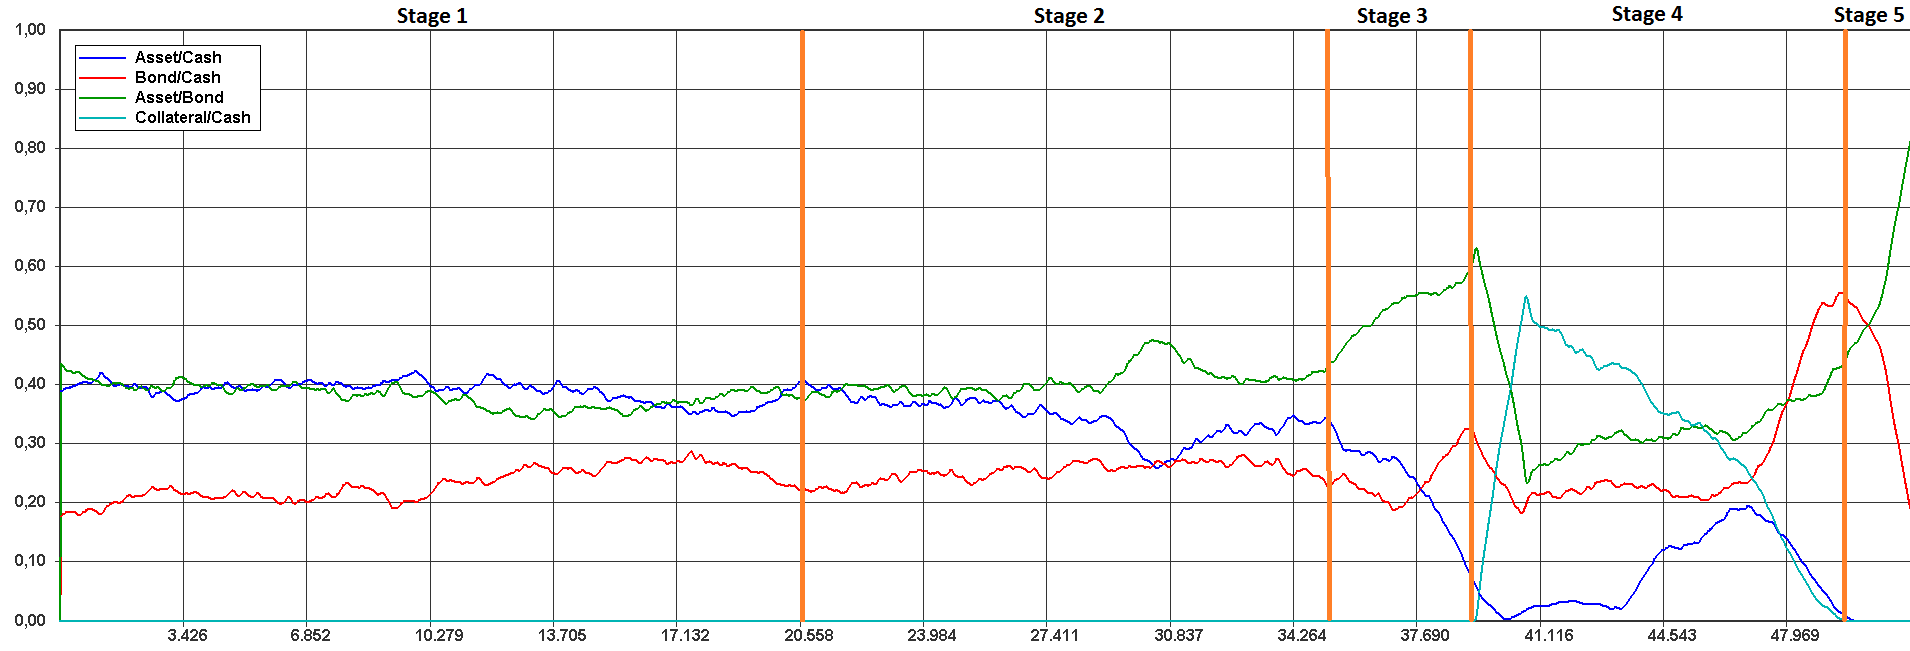
\includegraphics[width=1.0\textwidth, angle=0]{ac/ASCENDINGCONNECTED_100_DEFERREDCOLLATERALMARKET_MARKET_STAGES.png}
  	\caption{Market-activity stages of the single run of figure \ref{fig:wealth_ASCENDINGCONNECTED_100_DEFERREDCOLLATERALMARKET_SINGLE_FINAL}.}
	\label{fig:markets_ASCENDINGCONNECTED_100_DEFERREDCOLLATERALMARKET_MARKET_STAGES}
\end{figure}

Of course there are the same 3 stages to be found as described already in section \ref{sub:dynamics_singlerun} whereas the deferred enabling of the Collateral/Cash market adds 2 new stages.

\paragraph{Stage 4}
The free- and collateralized assets and bonds are traded by the pessimists towards the medianists and optimists and lead to a pattern similar to the end of stage 3.

\medskip

The Collateral/Cash market kicks in and allows the blocked goods to be traded again thus changing the activity of the other markets too. The Asset/Bond market initially drops rapidly just to recover shortly after. The Asset/Cash market previously dormant becomes active again because the pessimists have freed their collateral first because of selling it through the Collateral/Cash market and then through the Asset/Bond market or Bond/Cash market. Thus they have free assets they don't want and thus trade them against cash towards the medianists.

\begin{figure}[H]
	\centering
  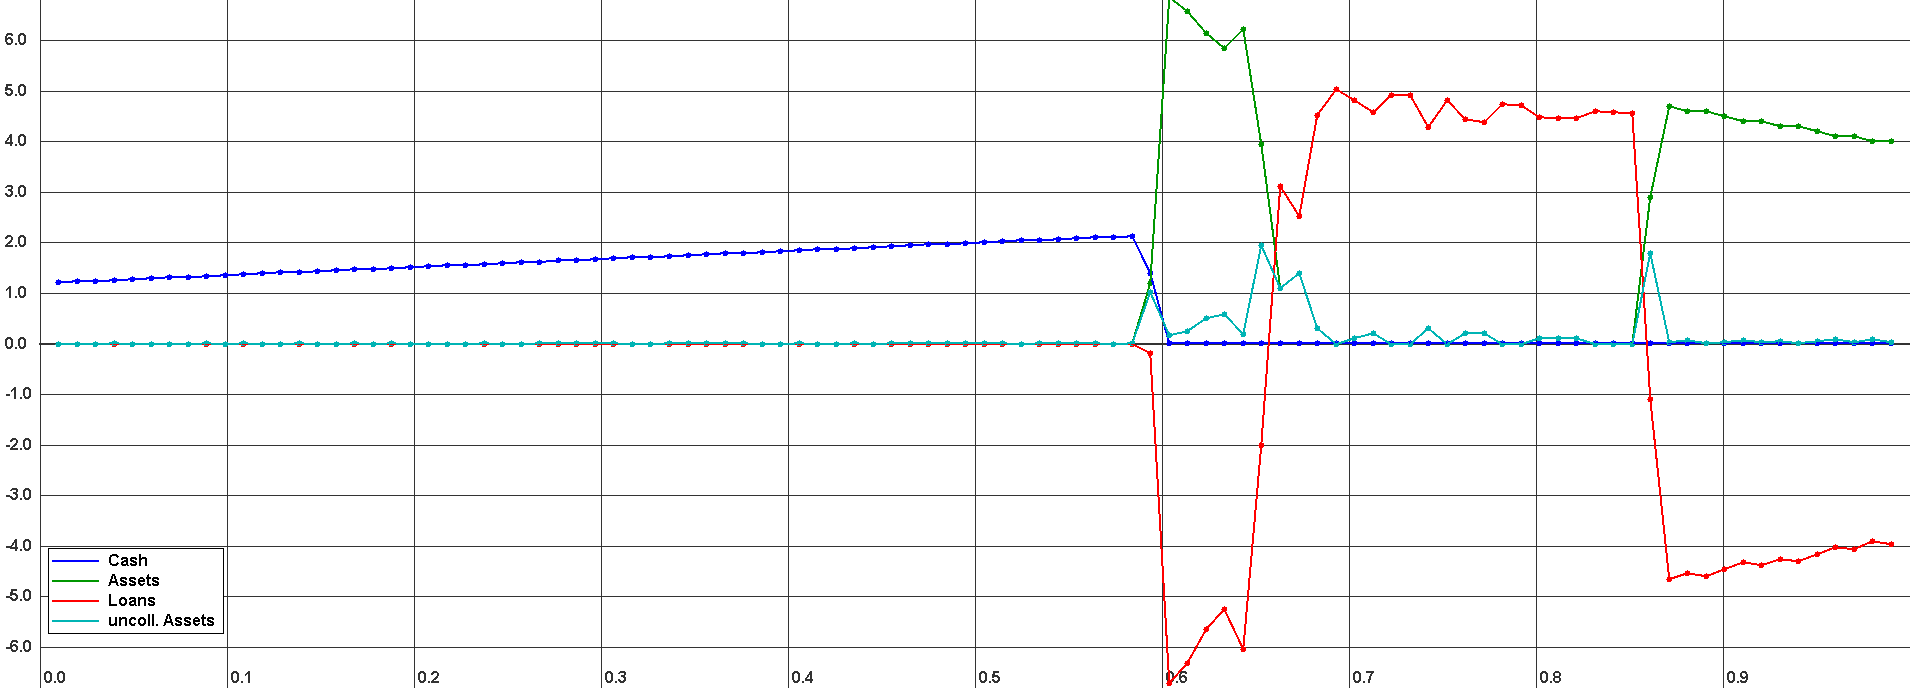
\includegraphics[width=1.0\textwidth, angle=0]{ac/ASCENDINGCONNECTED_100_DEFERREDCOLLATERALMARKET_WEALTH_STAGE_4.png}
  	\caption{Wealth-Distribution during Stage 4 of the single run of figure \ref{fig:wealth_ASCENDINGCONNECTED_100_DEFERREDCOLLATERALMARKET_SINGLE_FINAL}.}
	\label{fig:markets_ASCENDINGCONNECTED_100_DEFERREDCOLLATERALMARKET_WEALTH_STAGE_4}
\end{figure}

\paragraph{Stage 5}
The i1-point has finalized as no more pessimists are able to trade with their next medianists. Now only free assets in the range of medianists are traded towards the optimists which can only happen on the Asset/Bond market because both are out of cash. This will lead to the finalizing of the i2-point which can be seen in figure \ref{fig:wealth_ASCENDINGCONNECTED_100_DEFERREDCOLLATERALMARKET_SINGLE_FINAL}.
 
\begin{figure}[H]
	\centering
  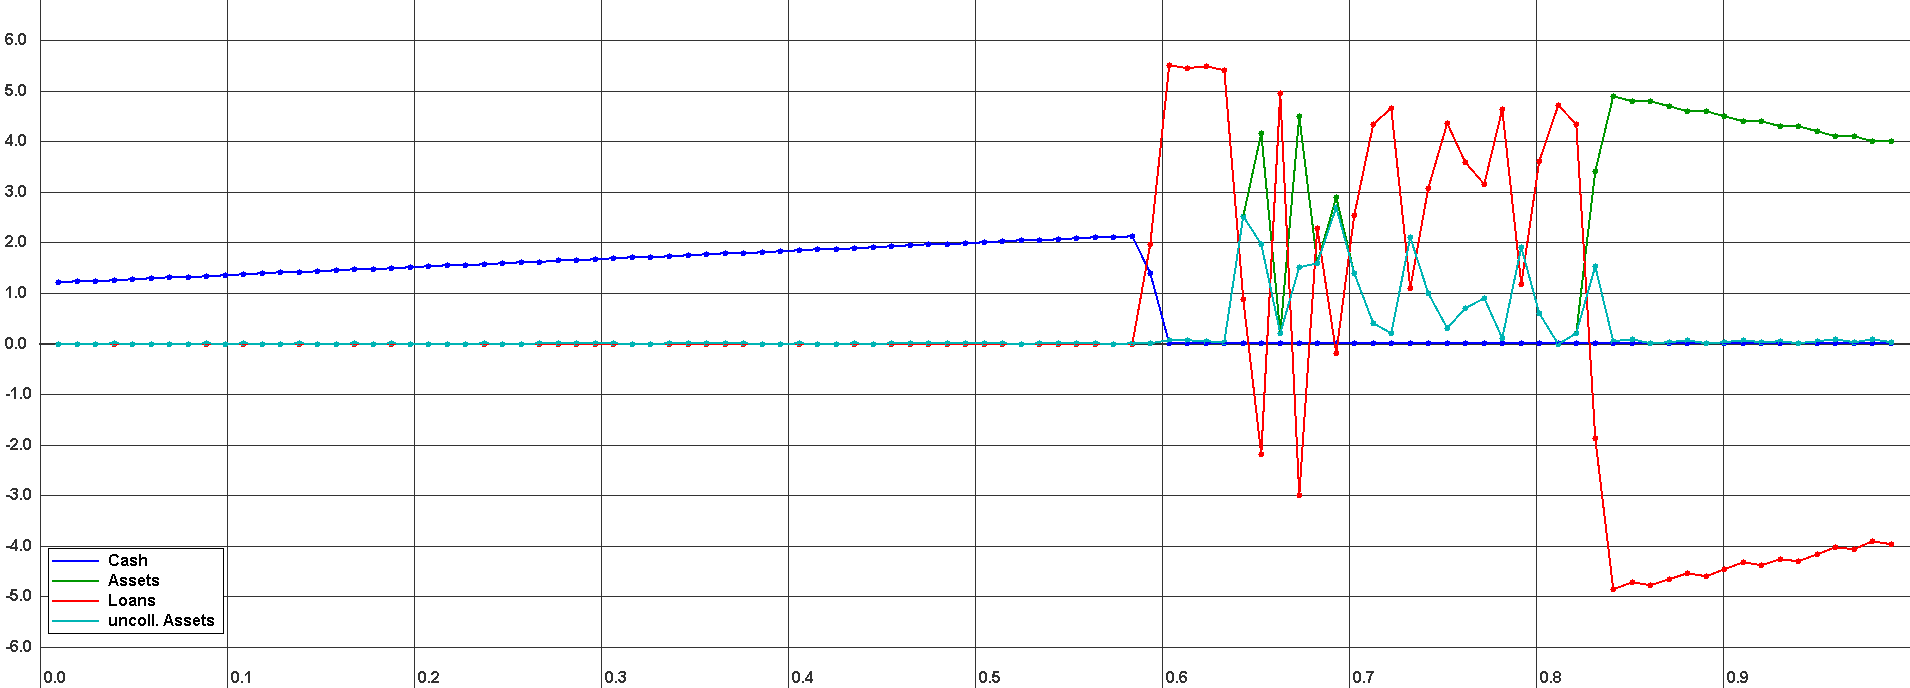
\includegraphics[width=1.0\textwidth, angle=0]{ac/ASCENDINGCONNECTED_100_DEFERREDCOLLATERALMARKET_WEALTH_STAGE_5.png}
  	\caption{Wealth-Distribution during Stage 5 of the single run of figure \ref{fig:wealth_ASCENDINGCONNECTED_100_DEFERREDCOLLATERALMARKET_SINGLE_FINAL}.}
  	\label{fig:markets_ASCENDINGCONNECTED_100_DEFERREDCOLLATERALMARKET_WEALTH_STAGE_5}
\end{figure}

\subsection{Ascending-Connected with new Market}

\begin{figure}[H]
	\centering
  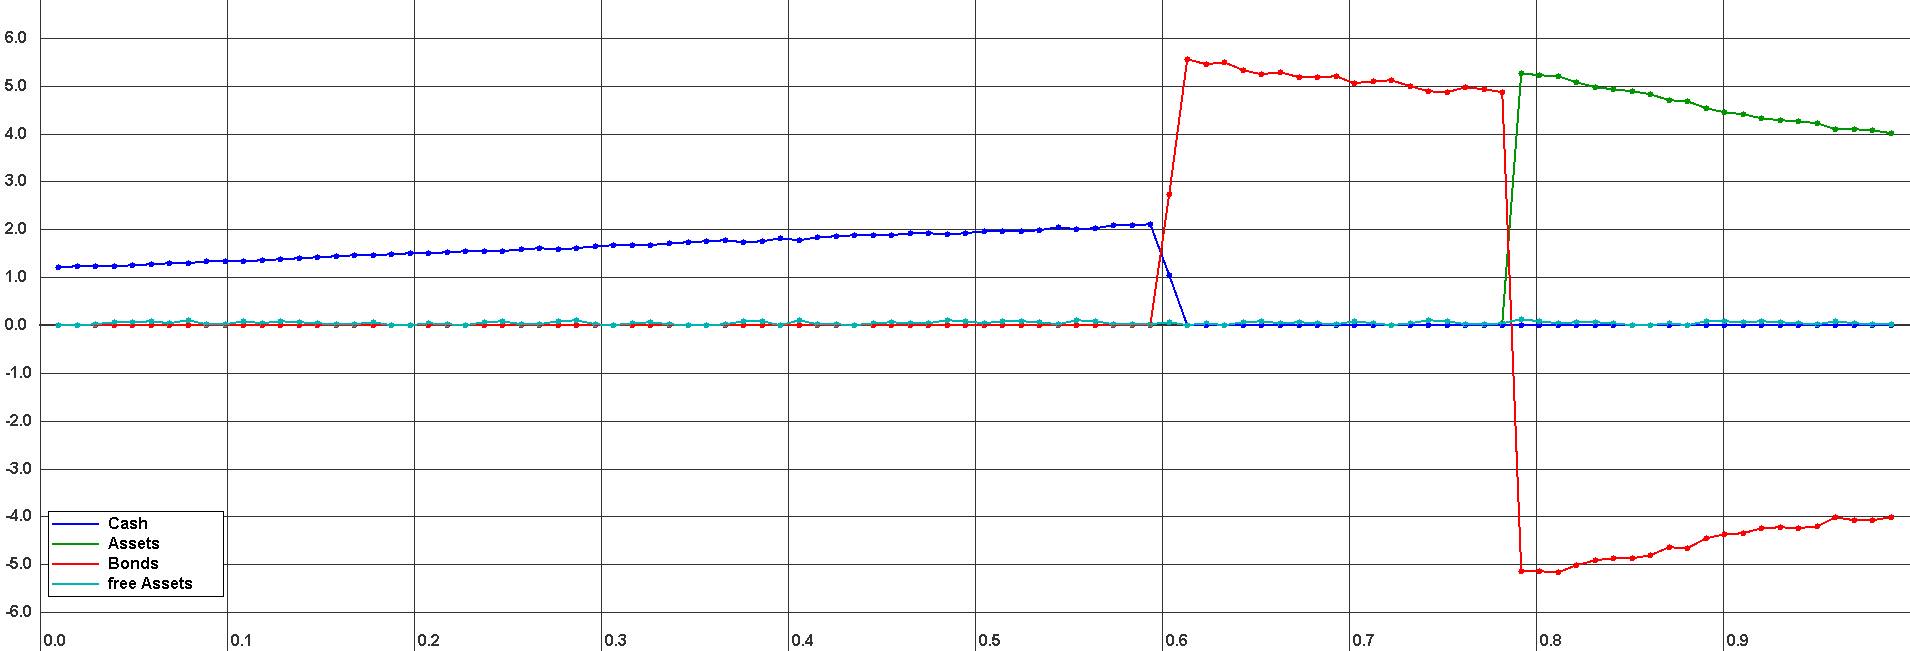
\includegraphics[width=1.0\textwidth, angle=0]{ac/ASCENDINGCONNECTED_100_WITHCOLLATERALMARKET_SINGLE.png}
  	\caption{Final wealth-distribution of a single run of Ascending-Connected topology with Collateral/Cash market enabled.}
	\label{fig:wealth_ASCENDINGCONNECTED_100_WITHCOLLATERALMARKET_SINGLE}
\end{figure}

\begin{figure}[H]
	\centering
  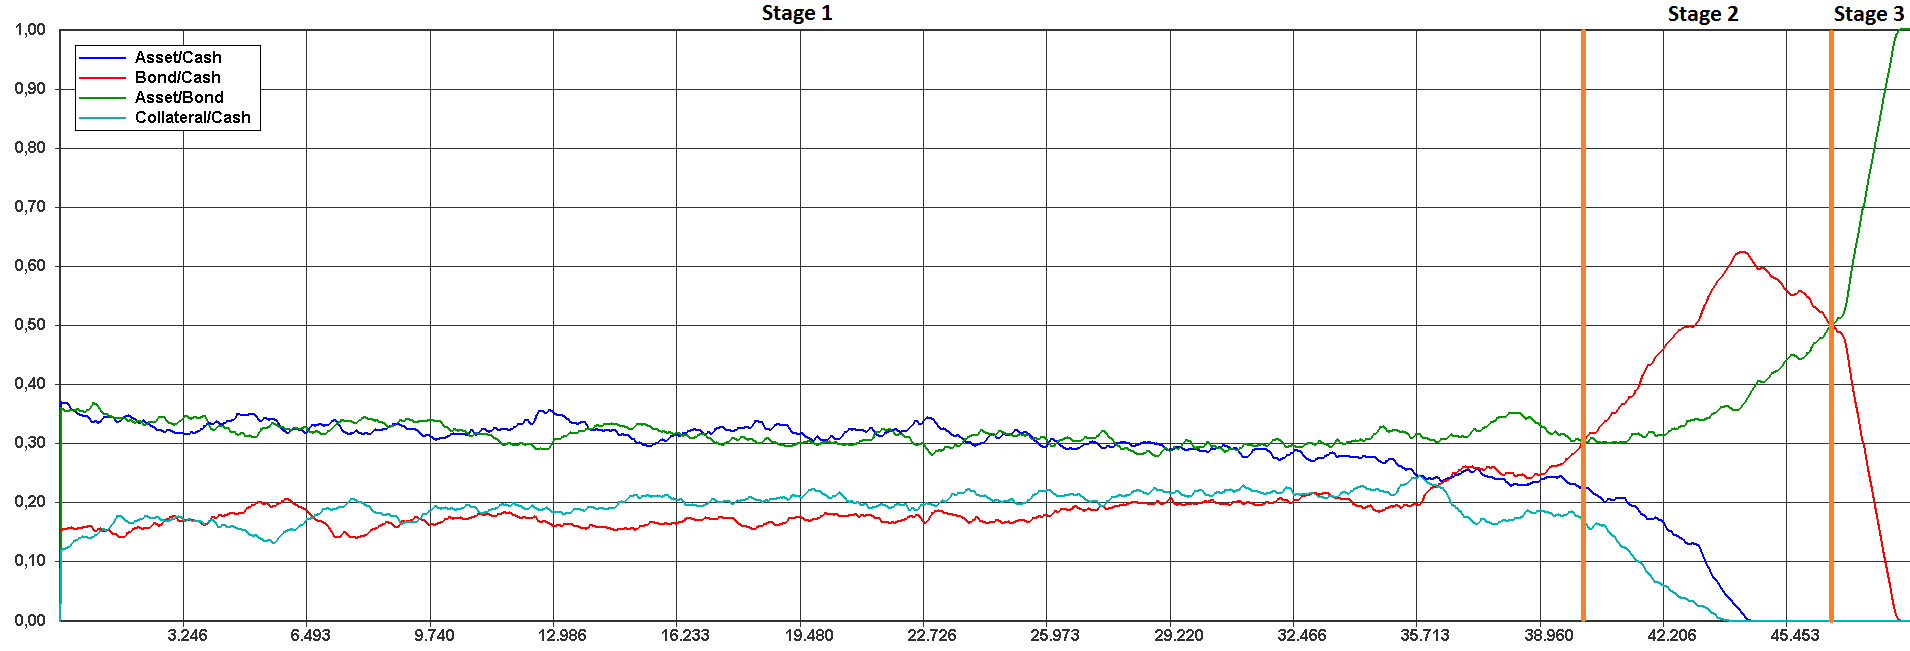
\includegraphics[width=1.0\textwidth, angle=0]{ac/ASCENDINGCONNECTED_100_WITHCOLLATERALMARKET_MARKET_STAGES.png}
  	\caption{Market-activity stages of the single run of figure \ref{fig:wealth_ASCENDINGCONNECTED_100_WITHCOLLATERALMARKET_SINGLE}.}
	\label{fig:markets_ASCENDINGCONNECTED_100_WITHCOLLATERALMARKET_MARKET_STAGES}
\end{figure}

3 stages were identified as can be seen in the Market-Dynamics diagram in figure \ref{fig:markets_ASCENDINGCONNECTED_100_WITHCOLLATERALMARKET_MARKET_STAGES}.

\paragraph{Stage 1}
Pessimists and optimists are emerge where the pessimists are gathering cash and selling all other goods. The optimists are buying assets against cash and against bonds. There are no medianists visible yet.

\medskip
The Bond/Cash market is slightly increasing as pessimists trade their bonds towards the later emerging medianists and the optimists. The Asset/Bond market is already very active as optimists trade assets against bonds after they have ran out of cash. Collateral/Cash market is rising slightly until the end where it drops as it is used by the pessimists to trade their collateral gathered on the other markets towards the optimists. The Asset/Cash market starts quite high because optimists trade their assets first towards the pessimists against cash but is declining slowly as fewer and fewer pessimists trade on this market.

\begin{figure}[H]
	\centering
  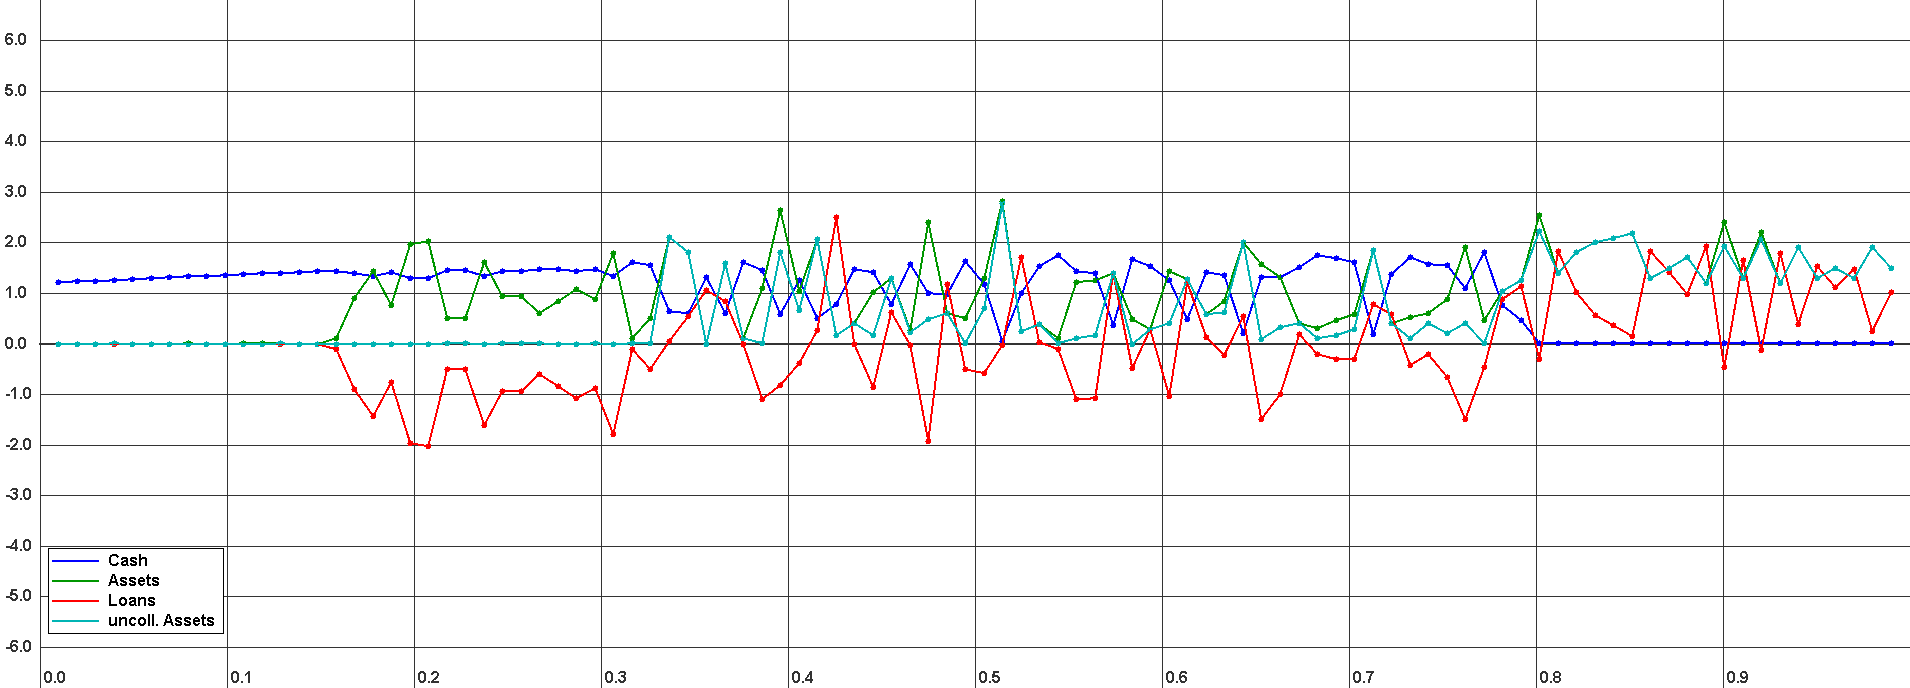
\includegraphics[width=1.0\textwidth, angle=0]{ac/ASCENDINGCONNECTED_100_WITHCOLLATERALMARKET_WEALTH_STAGE_1.png}
  	\caption{Wealth-Distribution during Stage 1 of the single run of figure \ref{fig:wealth_ASCENDINGCONNECTED_100_WITHCOLLATERALMARKET_SINGLE}.}
	\label{fig:wealth_ASCENDINGCONNECTED_100_WITHCOLLATERALMARKET_WEALTH_STAGE_1}
\end{figure}

\paragraph{Stage 2}
The pessimists are nearly final and hold only a few bonds which they trade towards the now emerging medianists. The medianists and optimists are approaching each other by trading towards the i2-point on the Asset/Bond market because both are out of cash and thus are only able to trade on this market with each other.

\medskip
Due to the remaining bonds in the pessimists range the Bond/Cash markets activity rises just to drop towards the end of this stage when all bonds have been traded up to the medianists and the pessimists have become dormant. The Asset/Bond market rises too due to increased activity between the medianists and optimists which can only trade between each other on this market because they are both out of cash making the other markets impossible choices. The Asset/Cash and Collateral/Cash markets activities decline as the pessimists which are the only agents which hold cash finally become inactive.

\begin{figure}[H]
	\centering
  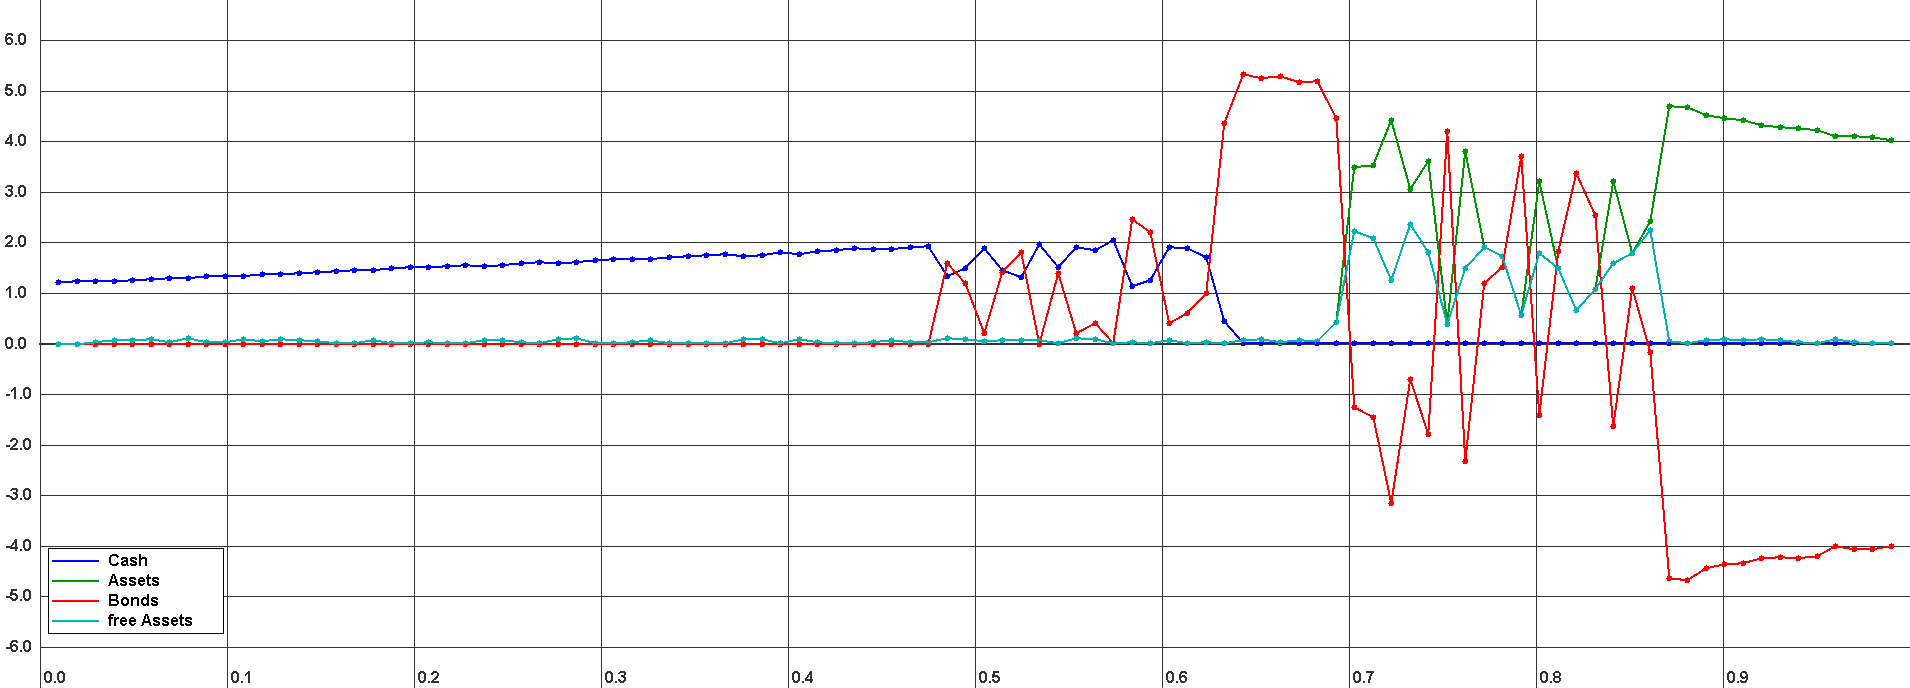
\includegraphics[width=1.0\textwidth, angle=0]{ac/ASCENDINGCONNECTED_100_WITHCOLLATERALMARKET_WEALTH_STAGE_2.png}
  	\caption{Wealth-Distribution during Stage 2 of the single run of figure \ref{fig:wealth_ASCENDINGCONNECTED_100_WITHCOLLATERALMARKET_SINGLE}.}
	\label{fig:wealth_ASCENDINGCONNECTED_100_WITHCOLLATERALMARKET_WEALTH_STAGE_2}
\end{figure}

\paragraph{Stage 3}
Pessimists are now final and won't change any more and the i1-point has emerged and is final. Medianists and optimists trade on the Asset/Bond market to finalize i2-point which can be seen in the final wealth-distribution in figure \ref{fig:wealth_ASCENDINGCONNECTED_100_WITHCOLLATERALMARKET_SINGLE}

\medskip
The only market which is active in this stage is the Asset/Bond market. The pessimists are already inactive and final thus generating no more activities on the Asset/Cash, Bond/Cash or Collateral/Cash markets. The medianists as well as the optimists have no more cash thus are only able to trade on the Asset/Bond market to finally trade the remaining assets in the range of the medianists towards the optimists until the i2-point has finalized.

\begin{figure}[H]
	\centering
  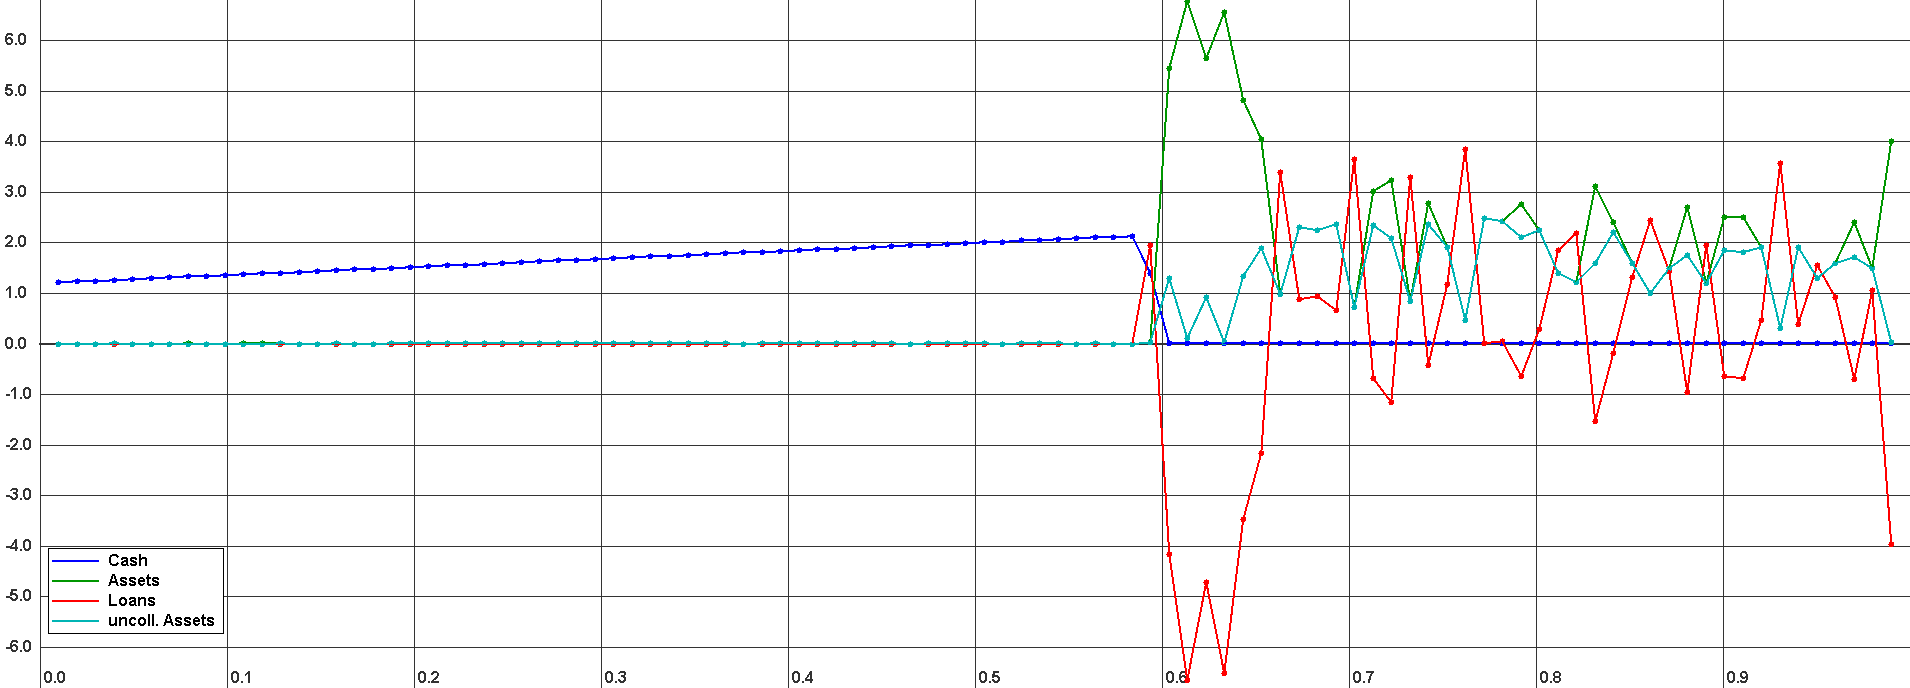
\includegraphics[width=1.0\textwidth, angle=0]{ac/ASCENDINGCONNECTED_100_WITHCOLLATERALMARKET_WEALTH_STAGE_3.png}
  	\caption{Wealth-Distribution during Stage 3 of the single run of figure \ref{fig:wealth_ASCENDINGCONNECTED_100_WITHCOLLATERALMARKET_SINGLE}.}
	\label{fig:wealth_ASCENDINGCONNECTED_100_WITHCOLLATERALMARKET_WEALTH_STAGE_3}
\end{figure}

After these observations made one can answer the questions.

\paragraph{Can the trading stages 1-4 be identified too as given in \cite{Breuer2015}?}
There are 4 stages in the case of both Fully-Connected and Ascending-Connected topology with the new market which are not the ones given in \cite{Breuer2015} but show up by pure chance and depend also a bit on the point-of-view on how to separate the stages from each other. 

\paragraph{How does trading progress with this new market? Is it the same as without the new market?}
The progression of the trading is obviously very different with the new market as compared to the market-activities without as the usage of the new market changes the dynamics completely.

\paragraph{How does the new market resolve the miss-allocation (with and without deferred activation)?}
It becomes active during the formation of the pessimists agents as they gather collateralized assets wealth which must be traded towards the optimists. The collateralized assets are traded from neighbour to neighbour until they reach the optimists-region.

\paragraph{When and how much is each market active?}
This can be seen clearly in the market-activity diagrams.

\paragraph{How do the market-activities change when a new market is introduced?}
They have less share on the overall activity and thus the new market is quite a heavy competitor in the overall share. The Asset/Bond market though is still the market on which the final trades occur.

\section{Conclusions on new Market}
The equilibrium of the Ascending-Connected topology with the new market is different than the Fully-Connected one which reaches the theoretical equilibrium. Thus the property of the hypothesis is still not sufficient because it predicted the Ascending-Connected topology to reach the theoretical equilibrium. This thesis can only speculate on the reason for this it is most probably rooted in the fundamental different trading dynamics of Ascending-Connected topology compared to Fully-Connected as can be seen in the market-dynamics. This thesis leaves the question of market-dynamics open for further research.

\end{document}
